
%(BEGIN_QUESTION)
% Copyright 2010, Tony R. Kuphaldt, released under the Creative Commons Attribution License (v 1.0)
% This means you may do almost anything with this work of mine, so long as you give me proper credit

Anta at en elektrisk aktuator brukes for å løfte en stor betongport i et vanningsanlegg. Porten fungerer i praksis som en reguleringsventil for vann i en åpen vanningskanal, og en kraftig vinsj styrer posisjonen:

$$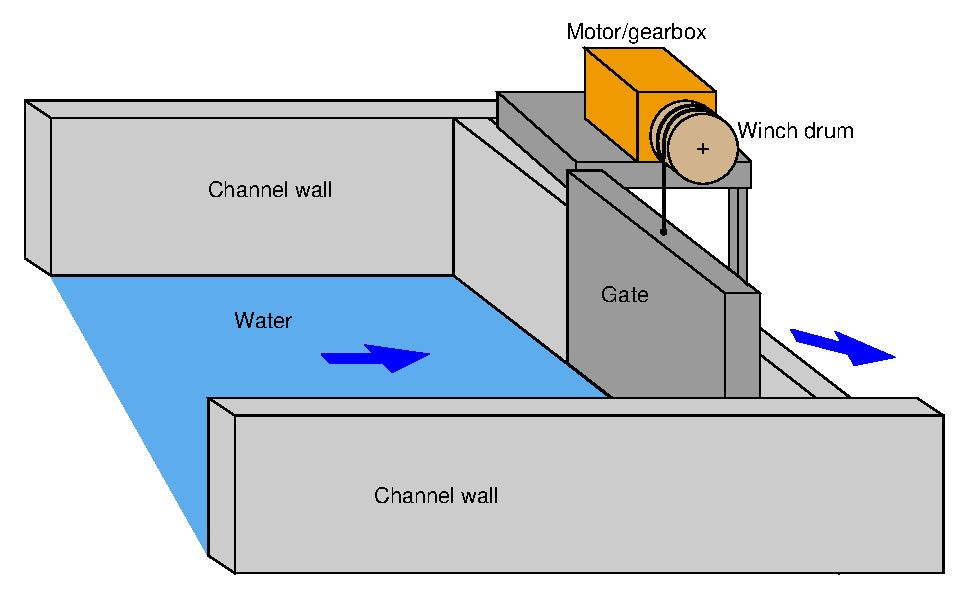
\includegraphics[width=15.5cm]{i00584x01.eps}$$

Vinsjtrommelen har diameter 20 tommer, og betongporten veier 12,740 pund. Beregn momentet som kreves på trommelen for å løfte porten, og momentet som kreves fra elmotoren når girutvekslingen er 1200:1.

Anta at elmotoren roterer med 1720 RPM (ved full last). Beregn vertikal løftehastighet for porten i fot per minutt. Beregn til slutt motorens utgangseffekt i horsepower ved denne lasten og hastigheten.

\vskip 20pt \vbox{\hrule \hbox{\strut \vrule{} {\bf Forslag til sokratisk diskusjon} \vrule} \hrule}

\begin{itemize}
\item{} Som i alle tekstoppgaver med beregning er det viktigste {\it hvordan} du kom fram til svaret, ikke bare tallverdiene. Forklar hvordan du satte opp ligningene for trommelmoment, motormoment, løftehastighet og motoreffekt.
\item{} En nyttig problemløsningsteknikk er å skissere et enkelt diagram av systemet. Selv når en figur allerede er gitt, kan en enklere skisse gjøre sammenhengene tydeligere. Lag en egen skisse og bruk den til å forklare løsningen.
\end{itemize}

\underbar{file i00584}
%(END_QUESTION)





%(BEGIN_ANSWER)

\noindent
{\bf Delvis svar:}

\vskip 10pt

$\tau_{motor}$ = 8.8472 lb-ft

\vskip 10pt

Motoreffekt ut = 2.897 horsepower

%(END_ANSWER)





%(BEGIN_NOTES)

Momentet på vinsjtrommelen er produktet av trommelradius og belastning. Radius er 10 tommer (0.8333 ft), som multiplisert med 12740 pund gir 10616.7 lb-ft moment på trommelen. Siden motoren driver trommelen gjennom 1200:1 reduksjon, trenger motoren bare 1/1200 av dette momentet, altså 8.8472 lb-ft.

\vskip 10pt

Motorhastigheten 1720 RPM reduseres av giret til trommelhastighet 1.4333 RPM. Hver trommelomdreining tilsvarer én omkrets lineær bevegelse av porten. Dermed blir løftehastigheten 1.4333 RPM $\times$ omkrets ($C = \pi d = 20\pi = 62.83$ tommer) = 90.06 tommer/min = 7.505 fot/min.

\vskip 10pt

Effekt er arbeid per tid. Arbeid per minutt er portvekt ganger løft per minutt: 12740 lb $\times$ 7.505 ft/min = 95612.6 ft-lb/min. Én horsepower er 550 ft-lb/s, og motoren leverer derfor 2.897 HP.

%INDEX% Fysikk, energi/arbeid/effekt: beregning av arbeid og effekt
%INDEX% Fysikk, moment: beregningsoppgave

%(END_NOTES)

